\documentclass{article}
\usepackage[paperwidth=20cm, paperheight=4cm, margin = 0cm, top=0.5cm]{geometry}
\usepackage{amsmath}


\usepackage{pgf}
\usepackage{tikz}


\usetikzlibrary{arrows,automata}

\tikzstyle{source}  = [draw,circle,fill=black,thick,inner sep=0mm,minimum size=2mm]

\renewcommand{\vec}[1]{\boldsymbol{#1}}

\begin{document}
\begin{center}
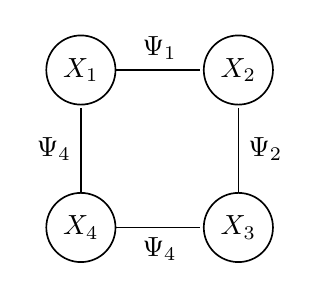
\begin{tikzpicture}[-,>=stealth',shorten >=1pt,auto,node distance=2cm,semithick]
                    
\node[state] (X1)               {$X_{4}$}; 
\node[state] (X2) [right of=X1] {$X_{3}$};                   

\node[state] (Y1) [above of=X1] {$X_{1}$}; 
\node[state] (Y2) [above of=X2] {$X_{2}$}; 

	
\path
	(X1) edge node[below]{$\Psi_4$} (X2)
	(Y1) edge node[above]{$\Psi_1$} (Y2);

\path
	(X1) edge node[left]{$\Psi_4$} (Y1)
	(X2) edge node[right]{$\Psi_2$} (Y2);


\end{tikzpicture}
\end{center}

\end{document}
